\documentclass[a4paper,12pt]{article}
\usepackage[utf8]{inputenc}
\usepackage[spanish]{babel}
\usepackage{graphicx}
\usepackage[margin=3cm]{geometry}
\usepackage{hyperref}
\usepackage{parskip}

\hypersetup{%
    pdfborder = {0 0 0}
}

\date{}

\title{\textbf{La paradoja de Aquiles y la Tortuga}}

\author{\begin{tabular}{rl}
  \textbf{Autor:} & Alba Puelles López \\
  \textbf{Correo:} & alba.puelles@um.es \\
  \textbf{Grupo:} & 1.1 \\
  \textbf{Profesor:} & Alberto Ruiz García \\
\end{tabular}}

\begin{document}
 
   \maketitle
   
   \newpage

   \tableofcontents

   \newpage
   
   \section{Introducción}
   
   En este documento presentaremos una paradoja que intenta contradecir
   el siguiente hecho: un corredor veloz alcanzará a uno lento aunque le dé ventaja. 
   
   Definiremos y desmostraremos la Paradoja de Aquiles desde un punto 
   de vista matemático porque como bien sabemos, mirándolo desde la física 
   (un corredor muy rápido puede adelantar a uno más lento aunque le de ventaja) 
   o hipotetizando algunas situaciones que pudieran pasar como que el corredor 
   lento se quedara sin aliento y abandonara la carrera, el rápido sí que podría ganar 
   la carrera. Análogamente, también sabemos que el corredor lento podría ganar 
   la carrera si al corredor rápido le sucediese algún contratiempo. 
   
   También definiremos y demostraremos su contraparadoja, que dice que el 
   corredor veloz tiene que conseguir alcanzar en algún punto al lento.
   
   \section{Definición del problema}
   
   Aquiles, conocido como ``el de los pies ligeros" debido a que se le consideraba 
   el hombre más veloz, decide participar en una carrera contra una tortuga. 
   Debido a que Aquiles es mucho más rápido, siendo capaz de recorrer 100 m. en 10 segundos, 
   decide darle una gran ventaja inicial de 100 metros a la tortuga que es diez 
   veces más lenta que él. 
   
   \section{Demostración}
   
   Al comienzo de la carrera, Aquiles recorre en poco tiempo los 100 m. 
   de ventaja que le había dejado a la tortuga, pero al llegar descubre 
   que la tortuga ya no está, sino que ha avanzado, más lentamente,
   10 m. más. 
   
   \begin{figure}[h]
   \begin{center}
   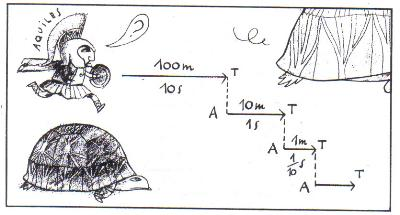
\includegraphics[width=8cm]{Imagenes/aquiles2.jpg}
   \end{center}
   \caption{Aquiles y la Tortuga}
   \label{fig:playa}
   \end{figure}
   
   Muy decidido y con ánimo, sigue corriendo, pero al alcanzar los 10m.
   que había avanzado la tortuga, ésta ha avanzado 0'1 m. más.  
   De esta manera, Aquiles nunca consigue ganar la carrera, ya que la tortuga
   siempre estará por delante de él. 
   
   A continuación se muestran las distancias recorridas por cada uno de ellos. Podemos
   comprobar que las distancias recorridas por ambos personajes representan
   series geométricas.
   
   Tomando como referencia la distancia recorrida por la tortuga obtenemos:
   
   \begin{equation}
   Tortuga = 100 + 10 + \frac{1}{10} + \frac{1}{100} + \frac{1}{1000} + ... = 10 \cdot \sum_{n=0}^\infty (\frac{1}{10})^n
   \end{equation}

   \begin{table}[h]
   \begin{center}
   \begin{tabular}{|l|l|l|l|l|}
   \hline
                     & \textbf{Pos. Aquiles (m.)} &  \textbf{Pos Tortuga (m.)}  & \textbf{Ventaja (m.)} & \textbf{T (s.)} \\ \hline
   \textbf{Salida}   & 0                          &  100                        & 100                   & 0                \\ \hline
   \textbf{1ª etapa} & 100                        &  100 + 10 = 110             & 10                    & 10               \\ \hline
   \textbf{2ª etapa} & 100 + 10 = 110             &  110 + 1 = 111              & 1                     & 10 + 1 = 11      \\ \hline 
   \textbf{3ª etapa} & 10 + 1 = 111               &  111 + 0'1 = 111'1          & 0'1                   & 11 + 0'1 = 11'1  \\ \hline 
   \textbf{...}      & ...                        &  ...                        & ...                   & ...              \\ \hline 
 
   \end{tabular}
   \end{center}
   \caption{Tabla de recorrido}
   \label{tab:ejemplo}
   \end{table} 

   Como podemos observar, la Tortuga siempre lleva una pequeña ventaja sobre Aquiles, pero, ¿es ésto cierto?,
   ¿qué pasa cuando la distancia que recorre cada uno tiende a infinito?, 
   En la siguiente sección veremos que los dos corredores tienen que cruzarse en un mismo punto del recorrido.
   
   \section{Demostración de la falsedad de la hipótesis}
   
   Es evidente pensar, como hemos comentado en la introducción del trabajo, que Aquiles
   debería de alcanzar en algún punto a la tortuga y que por lo tanto, algo había
   en aquella idea que no funcionaba. 
   
   \begin{figure}[h]
   \begin{center}
   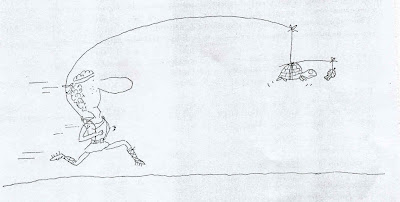
\includegraphics[width=8cm]{Imagenes/aquiles-tortuga.jpg}
   \end{center}
   \caption{Aquiles y la Tortuga}
   \label{fig:aquiles}
   \end{figure} 
    
   \newpage
   
   No fue hasta 24 siglos después de haber sido razonada la paradoja que, 
   gracias a la teoría de límites, se encontró el fallo que escondía,
   y es que la suposición de que infinitos trayectos deben sumar una distancia infinita en 
   un tiempo infinito no es correcta. Sabiendo ésto, cabe preguntarse lo siguiente,      
   ¿podemos encontrar un valor L para el cuál la siguiente expresión converja?: 
   
   \begin{equation}
   \lim\limits_{n \rightarrow \infty} 10 \cdot \sum_{n=0}^\infty (\frac{1}{10})^n = L
   \end{equation}   
   
   Partiendo de la serie anterior obtenemos la siguiente expresión:
   
   \begin{equation}
   \lim\limits_{n \rightarrow \infty} a \cdot \frac{(1 - r^n)}{1 - r}
   \end{equation}
   
   Sabemos que el límite cuando -1 $<$ r $<$ 1 es igual a 0 y en nuestro caso, r se encuentra en
   dicho intervalo (r = $\frac{1}{10}$). Además, sabemos que a = 100. Por tanto, 
   
   \begin{equation}
   \lim\limits_{n \rightarrow \infty} S_n = \frac{a}{1 - r} = \frac{100}{1 - \frac{1}{10}} = 111.11
   \end{equation}
   
   Hemos comprobado que la serie converje y que, por lo tanto, la hipótesis de Zenón era falsa,
   teniendo que alcanzar Aquiles a la Tortuga a los 111.11 m.
      
   \newpage
   
   \begin{thebibliography}{99}
   
      \bibitem{Wikipedia} https://es.wikipedia.org/wiki/Paradojas\_de\_Zenon
      \bibitem{HistoriaZenon} http://www.catedu.es/matematicas\_mundo/HISTORIA/historia\_Zenon.htm
      \bibitem{entremateymaticas}http://entremateymaticas.blogspot.com.es/2012/09/y-despues-de-dos-mil-anos.html
      
      
   \end{thebibliography}
  
\end{document} 
